
\newcommand{\printfigGraphTypes}{
    \begin{figure}
        \begin{subfigure}{.5\textwidth}
            \centering
            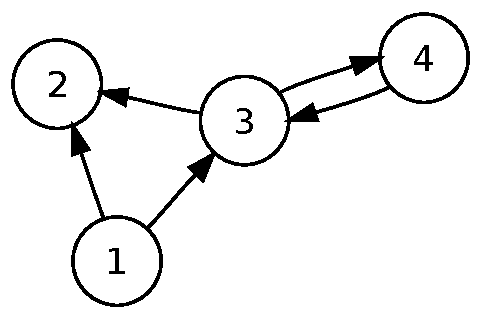
\includegraphics[width=.8\linewidth]{assets/images/Directed_graph_no_background.svg.pdf}
            \caption{Directed graph with cycle between nodes three and four.}
            \label{fig:directedgraph}
        \end{subfigure}
        \begin{subfigure}{.5\textwidth}
            \centering
            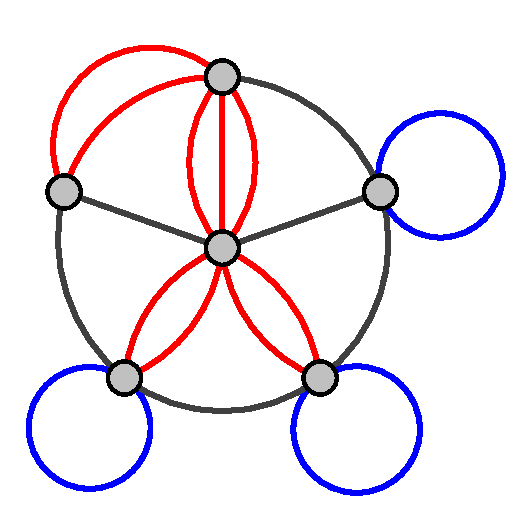
\includegraphics[width=.8\linewidth]{assets/images/Multi-pseudograph.svg.pdf}
            \caption{Multigraph with parallel edges and self-loops}
            \label{fig:multigraph}
        \end{subfigure}%
        \caption{Examples of first order graph symantics supported by Jaseci. (Images credits to wiki contributors~\cite{wiki:Directed_graph_no_background.svg,wiki:Multi-pseudograph.svg})}
        \label{fig:fig}
    \end{figure}
}